    \documentclass[11pt,
        usenames, % allows access to some tikz colors
        dvipsnames % more colors: https://en.wikibooks.org/wiki/LaTeX/Colors
    ]{report}
    \usepackage{
        amsmath,
        amssymb,
        fouriernc, % fourier font w/ new century book
        fancyhdr, % page styling
        lastpage, % footer fanciness
        hyperref, % various links
        setspace, % line spacing
        amsthm, % newtheorem and proof environment
        mathtools, % \Aboxed for boxing inside aligns, among others
        float, % Allow [H] figure env alignment
        enumerate, % Allow custom enumerate numbering
        graphicx, % allow includegraphics with more filetypes
        wasysym, % \smiley!
        upgreek, % \upmu for \mum macro
        listings, % writing TrueType fonts and including code prettily
        tikz, % drawing things
        booktabs, % \bottomrule instead of hline apparently
        cancel % can cancel things out!
    }
    \usepackage[margin=1in]{geometry} % page geometry
    \usepackage[
        labelfont=bf, % caption names are labeled in bold
        font=scriptsize % smaller font for captions
    ]{caption}
    \usepackage[font=scriptsize]{subcaption} % subfigures

    \newcommand*{\scinot}[2]{#1\times10^{#2}}
    \newcommand*{\bra}[1]{\left<#1\right|}
    \newcommand*{\ket}[1]{\left|#1\right>}
    \newcommand*{\dotp}[2]{\left<#1\,\middle|\,#2\right>}
    \newcommand*{\rd}[2]{\frac{\mathrm{d}#1}{\mathrm{d}#2}}
    \newcommand*{\pd}[2]{\frac{\partial#1}{\partial#2}}
    \newcommand*{\rtd}[2]{\frac{\mathrm{d}^2#1}{\mathrm{d}#2^2}}
    \newcommand*{\ptd}[2]{\frac{\partial^2 #1}{\partial#2^2}}
    \newcommand*{\md}[2]{\frac{\mathrm{D}#1}{\mathrm{D}#2}}
    \newcommand*{\norm}[1]{\left|\left|#1\right|\right|}
    \newcommand*{\abs}[1]{\left|#1\right|}
    \newcommand*{\pvec}[1]{\vec{#1}^{\,\prime}}
    \newcommand*{\svec}[1]{\vec{#1}\;\!}
    \newcommand*{\bm}[1]{\boldsymbol{\mathbf{#1}}}
    \newcommand*{\expvalue}[1]{\left<#1\right>}
    \newcommand*{\ang}[0]{\text{\AA}}
    \newcommand*{\mum}[0]{\upmu \mathrm{m}}
    \newcommand*{\at}[1]{\left.#1\right|}

    \newtheorem{theorem}{Theorem}[section]

    \let\Re\undefined
    \let\Im\undefined
    \DeclareMathOperator{\Res}{Res}
    \DeclareMathOperator{\Re}{Re}
    \DeclareMathOperator{\Im}{Im}
    \DeclareMathOperator{\Log}{Log}
    \DeclareMathOperator{\Arg}{Arg}
    \DeclareMathOperator{\Tr}{Tr}
    \DeclareMathOperator{\E}{E}
    \DeclareMathOperator{\Var}{Var}
    \DeclareMathOperator*{\argmin}{argmin}
    \DeclareMathOperator*{\argmax}{argmax}
    \DeclareMathOperator{\sgn}{sgn}
    \DeclareMathOperator{\diag}{diag\;}

    \DeclarePairedDelimiter\p{\lparen}{\rparen}
    \DeclarePairedDelimiter\s{\lbrack}{\rbrack}
    \DeclarePairedDelimiter\z{\lbrace}{\rbrace}

    % \everymath{\displaystyle} % biggify limits of inline sums and integrals
    \tikzstyle{circ} % usage: \node[circ, placement] (label) {text};
        = [draw, circle, fill=white, node distance=3cm, minimum height=2em]
    \definecolor{commentgreen}{rgb}{0,0.6,0}
    \lstset{
        basicstyle=\ttfamily\footnotesize,
        frame=single,
        numbers=left,
        showstringspaces=false,
        keywordstyle=\color{blue},
        stringstyle=\color{purple},
        commentstyle=\color{commentgreen},
        morecomment=[l][\color{magenta}]{\#}
    }

\begin{document}

\def\Snospace~{\S{}} % hack to remove the space left after autorefs
\renewcommand*{\sectionautorefname}{\Snospace}
\renewcommand*{\appendixautorefname}{\Snospace}
\renewcommand*{\figureautorefname}{Fig.}
\renewcommand*{\equationautorefname}{Eq.}
\renewcommand*{\tableautorefname}{Tab.}

\onehalfspacing

\pagestyle{fancy}
\rfoot{Yubo Su}
\cfoot{\thepage/\pageref{LastPage}}

\title{Research Notes}
\author{Yubo Su}
\rhead{}

\maketitle

\tableofcontents

\newpage

\chapter{Preliminary Problems}

To get an intuition for how Dedalus and fluid mechanics works, we will solve
some toy problems. Recall fluid equations in the presence of a uniform
gravitational field $\vec{g} = -g\hat{z}$:
\begin{equation}
    \begin{split}
        \rd{\rho}{t} + \vec{\nabla} \cdot \vec{u} &= 0,\\
        \rd{\vec{u}}{t} + \frac{\vec{\nabla}P}{\rho} - \vec{g} &= 0.
    \end{split}\label{eq:fluid_eq}
\end{equation}

In the incompressible limit, $\rd{\rho}{t} = 0$, which implies $\vec{\nabla}
\cdot \vec{u} = 0$. We use subscripts to indicate perturbed quantities, $Q_0$ is
background and $Q_1$ is perturbed. We will generally use $\vec{u}_0 = 0$ unless
otherwise noted. We will also generally assume symmetry along all axes except
$z$ the vertical axis.

In the incompressible limit, the fluid equations become
\begin{equation}
    \begin{split}
        \vec{\nabla} \cdot \vec{u}_1 &= 0,\\
        \pd{\rho_1}{t} + u_{1z}\pd{\rho_0}{z} &= 0,\\
        \pd{\vec{u}_1}{t} + \frac{1}{\rho_0}\vec{\nabla}P_1
            + \frac{\rho_1 g \hat{z}}{\rho_0} &= 0.
    \end{split}\label{eq:lin.incomp}
\end{equation}
We have used $\vec{\nabla}P_0 = -\rho_0 g \hat{z}$ in the absence of
perturbations.

\section{Incompressible, No Gravity}

We note that in the no gravity limit that $\rho_1$ does not have an effect on
other dynamical variables, so the equations of motion we must solve are
\begin{equation}
    \begin{split}
        \vec{\nabla} \cdot \vec{u}_1 &= 0,\\
        \pd{\vec{u}_1}{t} + \frac{\vec{\nabla}P_1}{\rho_0} &= 0.
    \end{split}\label{eq:lin.no_g_eom}
\end{equation}
We can take the divergence of the momentum equation and substitute the
continuity equation to get $\nabla^2 P = 0$.

\subsection{Dirichlet BCs}

This is a Laplace equation, which we've solved countless times. Imposing
periodic boundary conditions in the $x$ direction and $P_1(z = L) = 0, P_1(z =
0) = \mathcal{P}(x, t)$, we obtain eigenfunctions
\begin{equation}
    \begin{split}
        P_{1, n}(x, z, t) &=
            \frac{\mathcal{P}_n(t)}{\sinh(k_nL)}e^{ik_nx}\sinh\p*{k_n(L - z)},\\
        u_{1x, n}(x, z, t) &=
            \int\limits^t -\frac{1}{\rho_0}\pd{P_{1, n}}{x}\;\mathrm{d}t,\\
        u_{1z, n}(x, z, t) &=
            \int\limits^t -\frac{1}{\rho_0}\pd{P_{1, n}}{z}\;\mathrm{d}t.
    \end{split}\label{eq:incomp_nog}
\end{equation}
We define $k_n = \frac{2\pi n}{L}, n \geq 0$ and $\mathcal{P}(x, t) =
\sum\limits_n \mathcal{P}_n(t)e^{ik_nx}$.

Thus, if we impose BCs $\mathcal{P}(x, t) = \sin \frac{2\pi x}{L}$ and start
with initial conditions such that all quantities are zero, we would expect after
transients die out that
\begin{equation}
    \begin{split}
        P(x, z, t) &= \frac{\sin \frac{2\pi x}{L}}{\sinh 2\pi}
            \sinh \p*{2\pi \frac{L - z}{L}},\\
        u_{1x}(x, z, t) &= -\frac{2\pi t}{L\rho_0}
            \frac{\cos \frac{2\pi x}{L}}{\sinh 2\pi}\sinh \p*{2\pi \frac{L -
                z}{L}},\\
        u_{1z}(x, z, t) &= +\frac{2\pi t}{L\rho_0}
            \frac{\sin \frac{2\pi z}{L}}{\sinh 2\pi}\cosh \p*{2\pi \frac{L -
                z}{L}}.
    \end{split}\label{eq:incomp_nog_sol}
\end{equation}
This is in good agreement with the results, presented in \autoref{fig:no_g}.
Note that $P$ is constant while $\vec{u}$ increases linearly in time, and we
observe the expected $\sim \sin x \sinh \frac{L - z}{z}$ dependence. In fact,
$u_{1x}, u_{1z}$ are exactly $\frac{2\pi}{10}$ at $t = 1$.
\begin{figure}[!h]
    \centering
    \begin{subfigure}{0.3\textwidth}
        \centering
        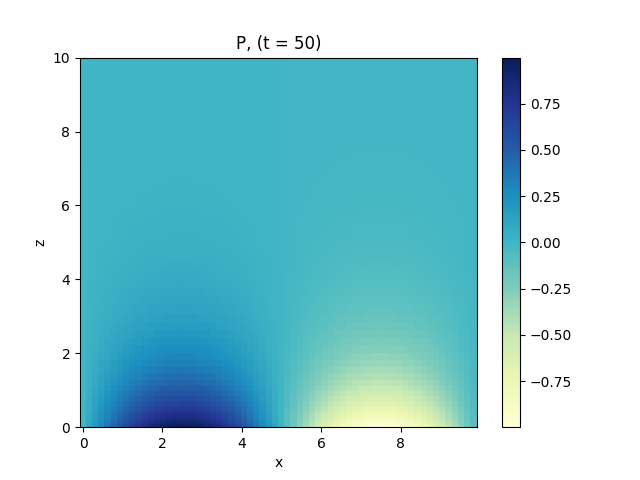
\includegraphics[width=\textwidth]{../sims/prelim/no_g/no_g_P_t50.png}
    \end{subfigure}
    \begin{subfigure}{0.3\textwidth}
        \centering
        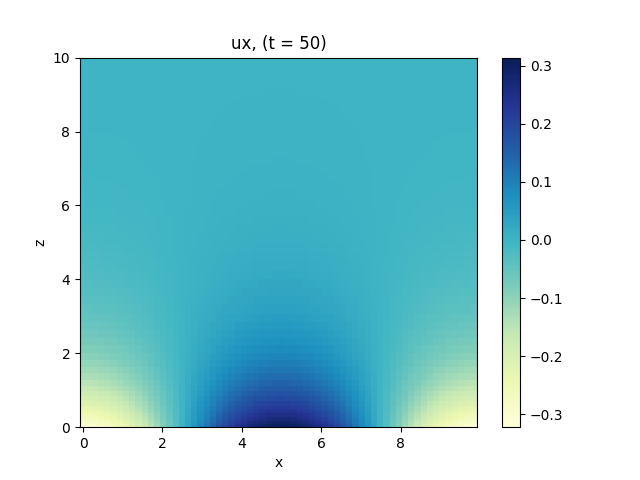
\includegraphics[width=\textwidth]{../sims/prelim/no_g/no_g_ux_t50.png}
    \end{subfigure}
    \begin{subfigure}{0.3\textwidth}
        \centering
        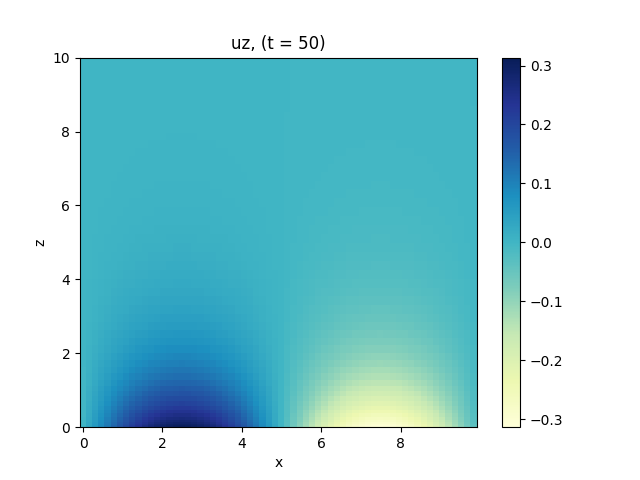
\includegraphics[width=\textwidth]{../sims/prelim/no_g/no_g_uz_t50.png}
    \end{subfigure}

    \begin{subfigure}{0.3\textwidth}
        \centering
        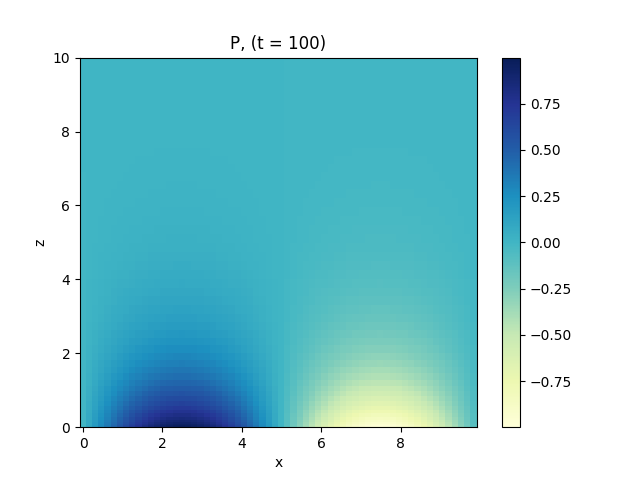
\includegraphics[width=\textwidth]{../sims/prelim/no_g/no_g_P_t100.png}
    \end{subfigure}
    \begin{subfigure}{0.3\textwidth}
        \centering
        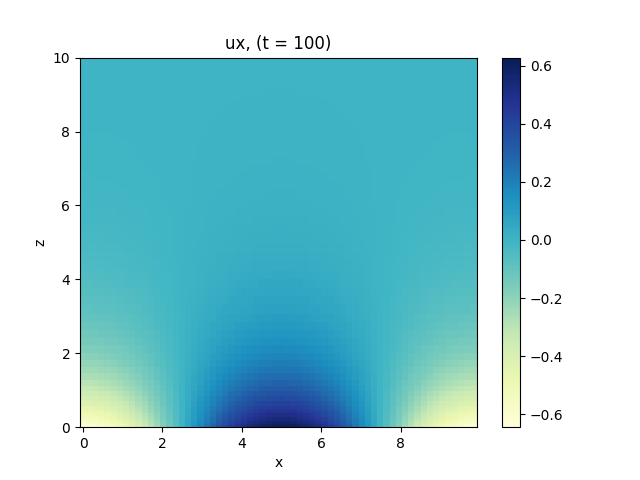
\includegraphics[width=\textwidth]{../sims/prelim/no_g/no_g_ux_t100.png}
    \end{subfigure}
    \begin{subfigure}{0.3\textwidth}
        \centering
        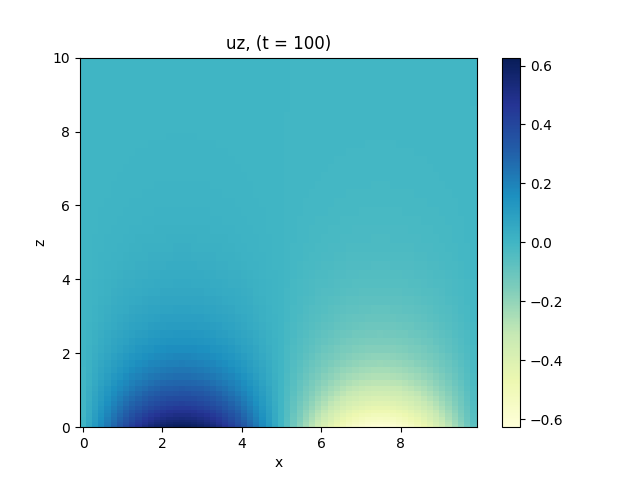
\includegraphics[width=\textwidth]{../sims/prelim/no_g/no_g_uz_t100.png}
    \end{subfigure}
    \caption{$P, u_x, u_z$ at $t = 0.5$ and $t = 1$ for $\rho_0 = 1$. We choose
    a $L = 10$ square domain.}\label{fig:no_g}
\end{figure}

\subsection{Things to Note}

It is worth noting that, since our \autoref{eq:lin.no_g_eom} reduced to a Laplace
equation, we needed two $z$ BCs and two $x$ BCs (periodic BCs amount to equating
the value and derivative of the function). This is in agreement with the
observation that the original \autoref{eq:lin.no_g_eom} had two derivatives in
$x, z$ apiece, so we needed two BCs each.

It is also worth seeing from our solution that $P$ immediately goes to the
equilibrium solution. This is not surprising since in the incompressible limit,
sound speed goes to infinity which is the timescale on which the pressure field
adjusts to net forces. Thus, the dynamics solely arise from the static pressure
field pushing the velocity field to equilibrium.

We chose time-independent $\mathcal{P}(x, t)$, but it is clear that whatever
$\mathcal{P}(x, t)$ we choose, the time dependence propagates to the velocities
by way of an integral. If we had instead chosen to take Fourier transform $t \to
\omega$, we would have had to integrate the boundary condition against the
eigenfunctions for each of the $\omega$, which is still easily computable, to
get the full $u_{1x}(x, z, t)$. We consider this in preparation for when we can
only solve for a set of $\vec{k}, \omega$ in the next problem.

The next thing we would have wanted to do is solve a problem with radiative BCs,
but we need to have wave solutions, which are missing in the absence of gravity.
We thus move on to the next configuration.

\section{Incompressible, Stratified w/ Gravity}

\subsection{Eigenfunctions}

Let's restore the $\rho_1 g$ term now. For funsies, we begin by solving for
arbitrary stratification $\rho_0(z)$ first. The fluid equations to first order
reduce to
\begin{equation}
    \begin{split}
        \pd{\rho_1}{t} + \p*{\vec{u}_1 \cdot \vec{\nabla}}\rho_0 &= 0,\\
        \vec{\nabla} \cdot \vec{u}_1 &= 0,\\
        \pd{\vec{u}_1}{t} &= -\frac{\vec{\nabla}P_1}{\rho_0}
            - \frac{\rho_1 g}{\rho_0}
    \end{split}\label{eq:lin_incomp}
\end{equation}
We expect there to be some $z$ dependence in the amplitude, so we substitute
variables of form $e^{i(kx - \omega t)}$ and do not specify the $z$ dependence.
This gives us
\begin{equation}
    \begin{split}
        -i\omega \rho_1 - u_{1z}\pd{\rho_0}{z} &= 0,\\
        iku_{1x} + \pd{u_{1z}}{z} &= 0,\\
        -iw u_{1x} + \frac{ik_x P_1}{\rho_0} &= 0,\\
        -iw u_{1z} + \frac{1}{\rho_0}\pd{P_1}{z} +
            \frac{\rho_1 g}{\rho_g} &= 0.
    \end{split}
\end{equation}
We substitute $N^2 = -\frac{g}{\rho_0}\pd{\rho_0}{z}$ to obtain
\begin{subequations}
    \begin{align}
        -i\omega \rho_1 - u_{1z}\frac{\rho_0N^2}{g} &= 0,\label{eq:lin.cont}\\
        iku_{1x} + \pd{u_{1z}}{z} &= 0,\label{eq:lin.div}\\
        -iw u_{1x} + \frac{ik_x P_1}{\rho_0} &= 0,\label{eq:lin.mom_x}\\
        -iw u_{1z} + \frac{1}{\rho_0}\pd{P_1}{z} +
            \frac{\rho_1g}{\rho_0} &= 0.\label{eq:lin.mom_z}
    \end{align}
\end{subequations}
Eliminating $u_{1x}$ by substituting~\eqref{eq:lin.div}
into~\eqref{eq:lin.mom_x} and $\rho_1$ by substituting~\eqref{eq:lin.cont}
into~\eqref{eq:lin.mom_z} give
\begin{subequations}
    \begin{align}
        i\omega \pd{u_{1z}}{z} + \frac{k_x^2 P_1}{\rho_0} &= 0,
            \label{eq:lin.eq1}\\
        \p*{\omega^2 - N^2 }u_{1z} + \frac{i\omega}{\rho_0}\pd{P_1}{z} &= 0.
            \label{eq:lin.eq2}
    \end{align}
\end{subequations}
Finally, we multiply~\eqref{eq:lin.eq1} with $\rho_0$ and differentiate
$\mathrm{d}z$ and combine with~\eqref{eq:lin.eq2} to give
\begin{equation}
    \rtd{u_{1z}}{z} + \frac{1}{\rho_0}\pd{\rho_0}{z}\pd{u_{1z}}{z}
        + k_x^2\p*{\frac{N^2}{\omega^2} - 1}u_{1z} = 0.\label{eq:lin.incomp.gen}
\end{equation}

Let's now pick stratification $\rho \propto e^{-z/H}$
\autoref{eq:lin.incomp.gen} clearly has exponential solutions $e^{\kappa z}$ for
\begin{equation}
    \kappa^2 - \frac{\kappa}{H} + k_x^2\p*{\frac{N^2}{\omega^2} - 1} = 0.
\end{equation}
We permit complex $\kappa = \frac{1}{2H} + ik_z$, and from the above clearly
\begin{align}
    k_z^2 &= -\frac{1}{4H^2} + k_x^2\p*{\frac{N^2}{\omega^2} - 1},\nonumber\\
    \omega^2 &= \frac{N^2k_x^2}{k_x^2 + k_z^2 +
        \frac{1}{4H^2}}.\label{eq:strat_disp}
\end{align}
Thus the eigenfunctions are
\begin{equation}
    \begin{split}
        u_{1z} &= e^{z/2H} e^{i(k_zz + k_xx - \omega t)},\\
        u_{1x} &= -\frac{k_z + i/2H}{k_x} u_{1z},\\
        \rho_1 &= \frac{i \rho_0}{H\omega} u_{1z},\\
        P_1 &= -\frac{\rho_0 \omega}{k_x^2}\p*{k_z + i/2H}u_{1z}.
    \end{split}\label{eq:strat_eigens}
\end{equation}

\subsection{Analytically Solving an IVP, Dirichlet + Driving BCs}

We will analyze everything in terms of $u_{1z}$ since it has the simplest form;
note that when actually choosing the BCs we will have to consider the gauge
freedom of $P$ and some considerations we defer to the computational section.

Currently, we have a set of eigenfunctions
\begin{equation}
    u_{1z}\p*{x, z, t \middle| \vec{k}, \omega}
        = e^{z/2H} e^{i(k_zz + k_xx - \omega t)}.
        \label{eq:strat.uz_eigen}
\end{equation}
Note that $u_{1z}$ is really only a function of two parameters rather than the
three $(k_x, k_z, \omega)$, since the three are related by dispersion relation
\autoref{eq:strat_disp}.

Now, we implement BCs. Consider domain $x, z \in [0, L]$. We will use periodic
BCs again in $x$, so then $k_{x, n} = \frac{2\pi n}{L}, n \geq 0$. Then, we will
require $u_{1z, n}(x, L, t) = 0$, a Dirichlet condition at the top boundary,
which restricts us to eigenfunctions of form
\begin{equation}
    u_{1z, n}\p*{x, z, t \middle| \vec{k}, \omega}
        = e^{z/2H}e^{i(k_xx - \omega t)}\sin\p*{k_z\p*{L - z}}.
        \label{eq:strat.uz_eigen_l-z}
\end{equation}

Finally, we must choose a BC at $z = 0$. We will choose a general function
$u_{1z}(x, 0, t) = F(x, t)$ where we can decompose
\begin{equation}
    F(x, t) = \int\limits \sum\limits_n \mathcal{F}(k_{x, n}, \omega)
        e^{i(k_{x, n}x - \omega t)}\;\mathrm{d}\omega.
\end{equation}
Matching BCs then gives us general solution for $u_{1z}$ given an arbitrary
driving function
\begin{equation}
    u_{1z}\p*{x, z, t \middle| \vec{k}, \omega}
        = \int\limits \sum\limits_n \mathcal{F}\p*{k_{x, n}, \omega}
            \frac{e^{z/2H}e^{i\p*{k_{x, n}x - \omega t}}\sin \p*{k_z(L - z)}}{
            \sin k_zL}\;\mathrm{d}\omega.
            \label{eq:strat.full_sol}
\end{equation}

For ease of computation, let's pick $F(x, t) = \cos \p*{\frac{2 \pi x}{L} -
\omega_0 t}$, so our full expected solution is (note $A + \epsilon =
Ae^{\epsilon/A} + \mathcal{O}(\epsilon^2)$)
\begin{equation}
    \begin{split}
        u_{1z}\p*{x, z, t \middle | \vec{k}, \omega}
            &= e^{z/2H}\frac{\cos\p*{\frac{2\pi x}{L} - \omega_0 t}
                \sin \p*{k_z(L - z)}}{\sin k_zL},\\
        u_{1x}\p*{x, z, t \middle | \vec{k}, \omega}
            &\approx -\frac{k_z}{k_x} e^{z/2H}\frac{
                \cos\p*{\frac{2\pi x}{L} - \omega_0 t + \frac{1}{2Hk_z}}
                \sin \p*{k_z(L - z)}
            }{\sin k_zL},\\
        \rho_1\p*{x, z, t \middle | \vec{k}, \omega}
            &\approx \frac{\rho_0}{H\omega} e^{z/2H}\frac{
                -\sin\p*{\frac{2\pi x}{L} - \omega_0 t}
                \sin \p*{k_z(L - z)}
            }{\sin k_zL},\\
        P_1\p*{x, z, t \middle | \vec{k}, \omega}
            &\approx -\frac{\rho_0 \omega k_z}{k_x^2} e^{z/2H}\frac{
                -\cos\p*{\frac{2\pi x}{L} - \omega_0 t + \frac{1}{2Hk_z}}
                \sin \p*{k_z(L - z)}
            }{\sin k_zL},\\
    \end{split}\label{eq:strat.part_sol}
\end{equation}
where $k_z: \omega(k_x, k_z) = \omega_0$ by the dispersion relation
\autoref{eq:strat_disp}. Note that $H$ contributes both to the overall
exponential profile and to the phase lag of $u_{1z}$.

\subsection{Computationally Solving an IVP, Dirichlet + Driving BCs}

To solve this computationally with the aforementioned BCs, periodic in $x$,
Dirichlet $0$ at $z = L$ and $\cos \p*{\frac{2\pi x}{L} - \omega_0 t}$ at $z =
0$, we must address the gauge freedom in $P$. This arises because for $k_x = 0$,
the divergence-free condition $\vec{\nabla} \cdot \vec{u}_1 = \pd{u_z}{z} = 0$
specificies $u_{1z}$ up to a constant already, so the bottom BC will fix the
value of $u_z$ when $k_x = 0$.

A different way of phrasing the same argument is as follows. Consider the
discrete $N \times N$ (square for notational simplicity) grid. At the boundary,
there is a list of values $f\p*{\z*{x_i}, z_0}$ that lives in an $N$ dimensional
space. We can thus pick a spanning set of $N$ basis vectors, and for each of
these $N$ vectors, by enforcing $\vec{\nabla} \cdot \vec{u} = 0$ at the boundary
we fix the allowed $f\p*{\z*{x_i}, z_{-1}}$ boundary conditions we can implement.
But there exists a choice of basis vectors for which one of the basis vectors is
constant $f_i\p*{\z*{x_i}, z_0} = C$. For this basis vector, the boundary
condition is fully determined, so we only have $N - 1$ dimensions from which to
choose the BCs $f\p*{\z*{x_i}, z_{-1}}$. Since the dimensionality of a space
cannot depend on the choice of basis vector, the divergence free condition
actually yields an extra degree of freedom.

We can use this extra degreee of freedom to specify $P(z = L) = 0$ so the
oscillations should have zero mean. Then we can just simulate away!

Since we're much more interested in the $z$ behavior, we will set the $z$ axis
to be further away. Let's choose $\rho_0 = 1, L_x = 10, L_z = 20, k_x = 2, k_z =
1, H = 5, g = 10$ which constrains $N^2 \equiv g/H = 1, \omega^2 = \frac{4}{5 +
1/100}$. Some considerations:
\begin{itemize}
    \item $\frac{1}{k_xH}, \frac{1}{k_zH}$ are $1/10, 1/5$ respectively,
        small-ish but $L_Z = 8H$ so we should be able to see the $e^{z/2H}$
        behavior well.

    \item The vertical phase velocity is $\frac{\omega}{k_z} \sim 1$, so we
        should simulate at least out to $t = 20$ for the wave to fully propagate
        to the boundary.
\end{itemize}

\subsection{Sommerfield/Radiative BCs}

\section{(Algebra) The Anelastic/Boussinesq Approximations}

\subsection{Developing the Anelastic/Boussinesq Approximations}

Let's relax the incompressibility constraint (we will expand the continuity
equation to first order, but the momentum equation will merit a separate
treatment):
\begin{equation}
    \begin{split}
        \pd{\rho_1}{t} + \vec{\nabla} \cdot \p*{\rho_0 \vec{u}_1} &= 0,\\
        \pd{\vec{u}_1}{t} &= -\frac{\vec{\nabla}P}{\rho} - \vec{g}.
    \end{split}
\end{equation}
Suppose we are interested in phenomena with characteristic length scale $L$ and
time scale $\tau$. Let's first examine the relative magnitudes of the terms in
the continuity equation
\begin{equation*}
    \frac{\rho_1}{\tau} + \frac{\rho_0 \abs{u_1}}{L} = 0.
\end{equation*}
Thus, if we are interested in time scales $\tau \gg
\frac{\rho_1}{\rho_0}\frac{L}{\abs{u_1}}$ then we neglect the first term, the
time derivative. This corresponds to making the perturbation incompressible;
note that $\pd{\rho_1}{t} \approx \rd{\rho_1}{t}$ to first order, so we drop the
high frequency restoring forces in the perturbation.

For the momentum equation, we instead first manipulate to first order
\begin{align}
    -\frac{\vec{\nabla}P}{\rho} - \vec{g}
        &= -\frac{\vec{\nabla}P_0}{\rho} - \frac{\vec{\nabla}P_1}{\rho_0}
            - \vec{g},\nonumber\\
        &= - \frac{\vec{\nabla}P_1}{\rho_0} +
            \p*{\frac{\rho_0}{\rho} - 1}\vec{g},\nonumber\\
        &= -\vec{\nabla}\p*{\frac{P_1}{\rho_0}}
            - \frac{P_1}{\rho_0^2}\vec{\nabla}\rho_0
            - \frac{\rho_1}{\rho_0}\vec{g}.
\end{align}

We now have three equations for four variables, $\vec{u}_1, \rho_1, P_1$. We
must introduce a fourth equation, a thermodynamic equation. For an adiabatic
process $P\rho^{-\gamma} \propto P^{1-\gamma}T^\gamma$ is constant. We thus
introduce the concept of the \emph{potential temperature}
\begin{equation}
    \theta = T\p*{\frac{P_0}{P}}^\kappa.
        \label{eq:pot_temp}
\end{equation}
For an adiabatic process, $\rd{\theta}{t} = 0$. Motivated by this, we use
\begin{equation}
    \begin{split}
        \pd{1}{\rho_0}\pd{\rho_0}{z} &= \frac{1}{\gamma P_0}\pd{P_0}{z}
            - \frac{1}{\theta_0}\pd{\theta_0}{z},\\
        \frac{\rho_1}{\rho_0} &= \frac{1}{\gamma} \frac{P_1}{P_0}
            - \frac{\theta_1}{\theta_0},
    \end{split}
\end{equation}
to give the momentum equation form
\begin{equation}
    \rd{\vec{u}_1}{t} = -\vec{\nabla}\p*{\frac{P_1}{\rho_0}}
        + \frac{P_1}{\rho_0}\p*{\frac{1}{\theta_0}\vec{\nabla}\theta_0}
        + \vec{g} \frac{\theta_1}{\theta_0}.\label{eq:mom_unsimp}
\end{equation}

We also recognize $N^2 = \frac{g}{\theta_0}\pd{\theta_0}{z}$. We now do the same
trick where we consider dynamics on length scale $D$ and compare the first and
second terms in \autoref{eq:mom_unsimp}. Their ratio is $\frac{N^2 D}{g}$, and
so as $N^2 \ll \frac{g}{D}$ the freefall time we neglect the second term.

The anelastic fluid equations thus read
\begin{equation}
    \begin{split}
        \vec{\nabla} \cdot \p*{\rho_0\vec{u}} &= 0,\\
        \pd{\vec{u}_1}{t} + \vec{\nabla}\p*{\frac{P_1}{\rho_0}}
            - \vec{g}\frac{\theta_1}{\theta_0} &= 0,\\
        \pd{\theta_1}{t} + \p*{\vec{u} \cdot \vec{\nabla}}\theta_0 &= 0.
    \end{split}\label{eq:lin_anelastic}
\end{equation}

The Boussinesq equations are obtained from these in the limit where $H \gg D$
the relevant length scale, thus we allow $\rho_0$ to be approximately constant.

\subsection{Anelastic Solution to Stratified Atmosphere}

We simply substitute $e^{i(\vec{k} \cdot \vec{r} - \omega t)}$ into
\autoref{eq:lin_anelastic} with $\rho_0 \propto e^{-z/H}$ and obtain
\begin{equation}
    \begin{bmatrix}
        0 & 0 & ik_x\rho_0 & ik_z \rho_0 - \frac{\rho_0}{H}\\
        0 & -i\omega & 0 & \frac{N^2\theta_0}{g}\\
        \frac{ik_x}{\rho_0} & 0 & -i\omega & 0\\
        \frac{ik_z}{\rho_0} + \frac{1}{\rho_0 H} & -\frac{g}{\theta_0}
            & 0 & -i\omega
    \end{bmatrix} \begin{bmatrix}
        P_1 \\ \theta_1 \\ u_{1x} \\ u_{1z}
    \end{bmatrix} = 0.
\end{equation}
Taking the determinant of this matrix produces
\begin{align}
    -k_x^2\p*{-N^2 + \omega^2} + \p*{ik_z - \frac{1}{H}}
        \p*{ik_z + \frac{1}{H}}\omega^2 &= 0,\nonumber\\
    \frac{N^2k_x^2}{k_x^2 + k_z^2 + \frac{1}{4H^2}} &= \omega^2.
\end{align}

\chapter{2D Wave Breaking in Atmospheres}

\section{Dynamical Setup}

TODO (fluid equations, driven on bottom, parameters)

\section{Boundary Conditions}

TODO (periodic in x, show that right number of BCs in $z$, discuss whether gauge
choice).

\section{Simulation}

TODO (CFL conditions etc.)

\end{document}

